\section{Modelo de arquitectura C4}

En el presente anexo se documenta la arquitectura de software de la plataforma \textbf{SocioUnido} utilizando el modelo C4. Este modelo permite visualizar el sistema desde distintos niveles de abstracción, facilitando la comprensión tanto para perfiles de negocio como para el equipo de desarrollo y operaciones.

A continuación, se presentan los diagramas correspondientes a los niveles de Contexto (Nivel 1), Contenedores (Nivel 2) y Componentes (Nivel 3) para los distintos microservicios que componen el ecosistema.

\subsection{Nivel 1 del modelo de arquitectura C4}

% Nivel 1: Contexto
\begin{figure}[h!]
    \centering
    % Nota: Las comillas en el nombre del archivo evitan errores de compilación por los espacios
    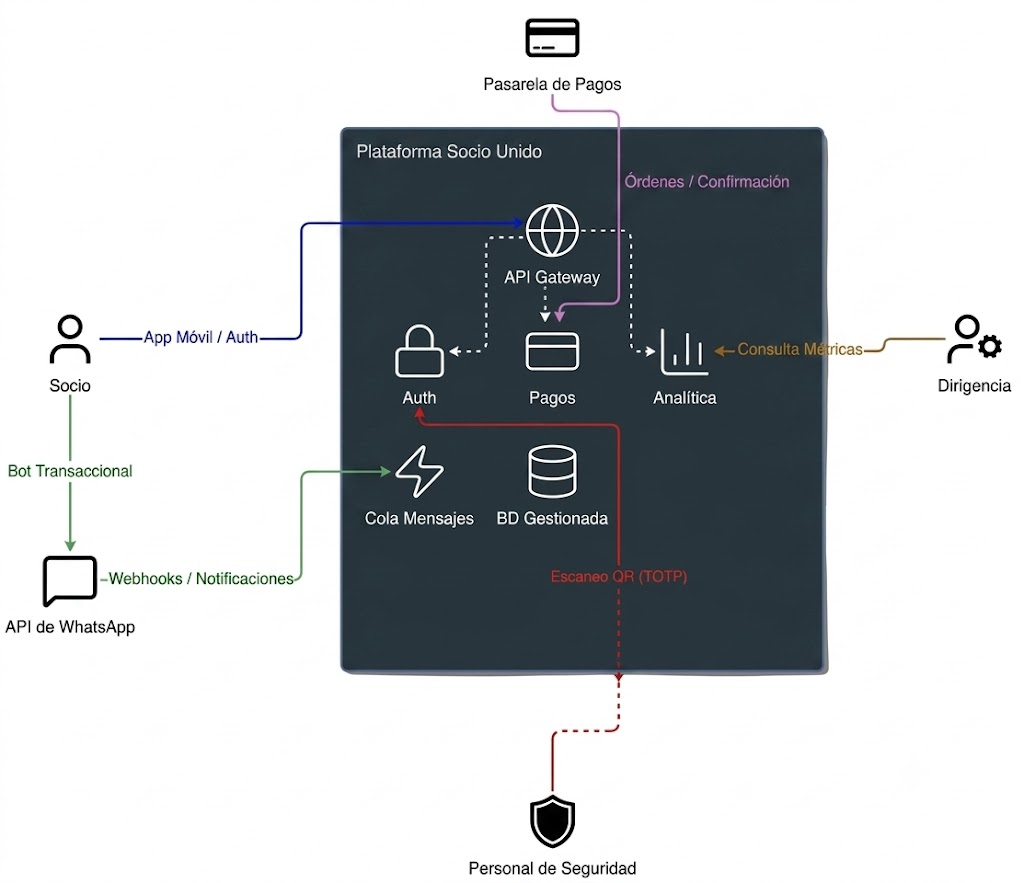
\includegraphics[width=\textwidth]{img/c4_model/C4 Nivel 1.jpg}
    \caption{Diagrama C4 nivel 1: Contexto del sistema. Interacción de la plataforma SocioUnido con los distintos actores (Socios, Dirigencia, Personal de Control) y sistemas externos (Pasarela de Pagos, Interfaz de Programación de Aplicaciones [API] de WhatsApp).}
    \label{fig:c4_nivel1}
\end{figure}

\newpage

\subsection{Nivel 2 del modelo de arquitectura C4}

% Nivel 2: Contenedores
\begin{figure}[h!]
    \centering
    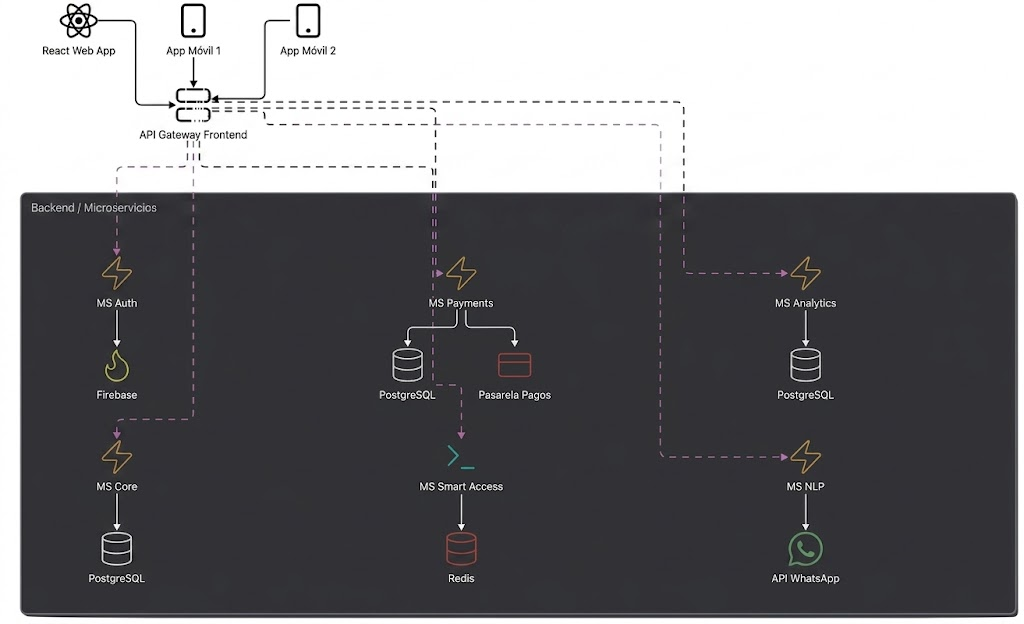
\includegraphics[width=\textwidth]{img/c4_model/C4 Nivel 2.png}
    \caption{Diagrama C4 nivel 2: Contenedores. Vista de alto nivel de las aplicaciones web, móviles, bases de datos y la arquitectura basada en microservicios detrás de la puerta de enlace de API (API Gateway).}
    \label{fig:c4_nivel2}
\end{figure}

\newpage

\subsection{Nivel 3 del modelo de arquitectura C4}

% Nivel 3: Componentes (MS Core / Gestión Societaria)
\begin{figure}[h!]
    \centering
    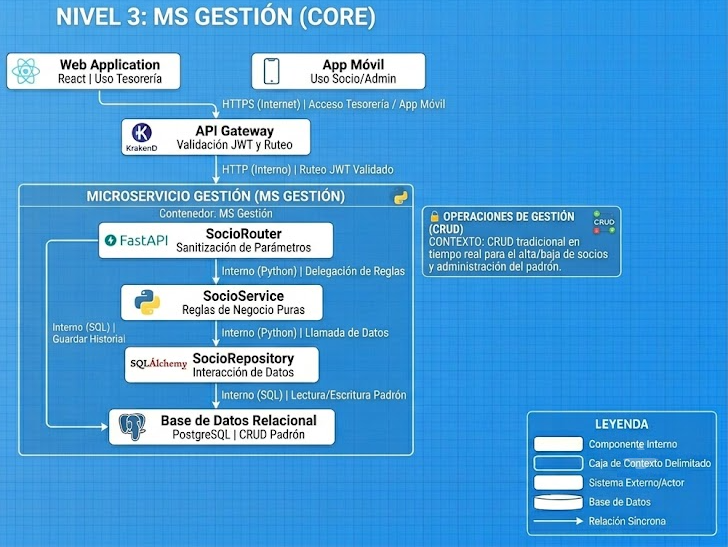
\includegraphics[width=\textwidth]{img/c4_model/C4 Nivel 3-MS Gestion.png}
    \caption{Diagrama C4 nivel 3: Componentes (Microservicio de gestión societaria). Detalle del microservicio principal encargado de la creación, lectura, actualización y borrado (CRUD) de usuarios, perfiles y reglas de negocio del padrón societario.}
    \label{fig:c4_nivel3_gestion}
\end{figure}

% Nivel 3: Componentes (MS NLP)
\begin{figure}[h!]
    \centering
    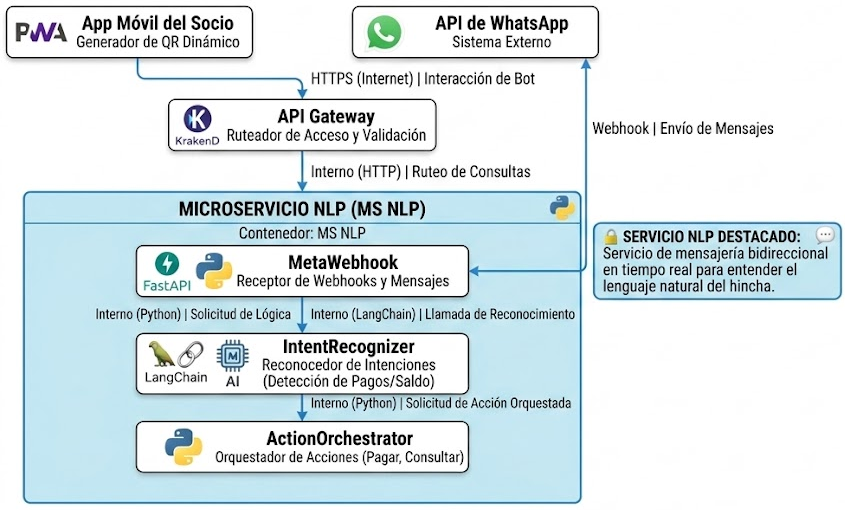
\includegraphics[width=\textwidth]{img/c4_model/C4 Nivel 3-MS NLP.png}
    \caption{Diagrama C4 nivel 3: Componentes (Microservicio de Procesamiento de Lenguaje Natural [PLN]). Detalle del motor de procesamiento de lenguaje natural integrado vía retrollamada web (Webhook) con la API de WhatsApp para la atención automatizada.}
    \label{fig:c4_nivel3_nlp}
\end{figure}

\newpage

% Nivel 3: Componentes (MS Payments)
\begin{figure}[h!]
    \centering
    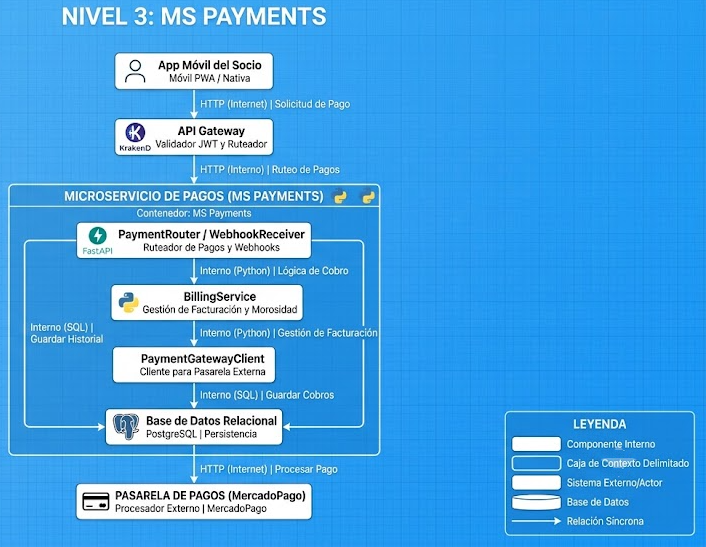
\includegraphics[width=\textwidth]{img/c4_model/C4 Nivel 3-MS Payments.png}
    \caption{Diagrama C4 nivel 3: Componentes (Microservicio de pagos). Arquitectura del componente encargado de la facturación y comunicación con pasarelas de pago externas.}
    \label{fig:c4_nivel3_payments}
\end{figure}

% Nivel 3: Componentes (MS Smart Access)
\begin{figure}[h!]
    \centering
    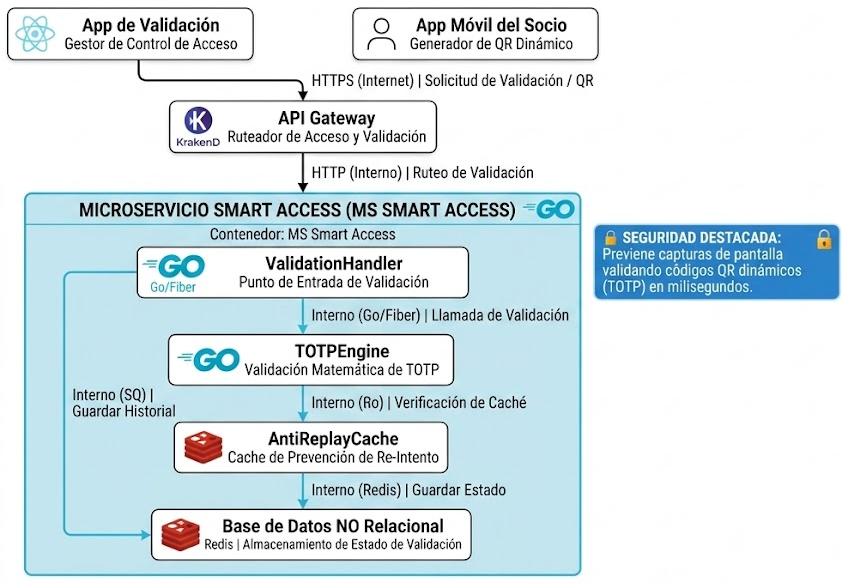
\includegraphics[width=\textwidth]{img/c4_model/C4 Nivel 3-MS Smart Access.png}
    \caption{Diagrama C4 nivel 3: Componentes (Microservicio de Acceso Inteligente). Lógica interna de validación matemática y fuera de línea (offline) mediante contraseñas de un solo uso basadas en el tiempo (TOTP) para el control de acceso en estadios.}
    \label{fig:c4_nivel3_smartaccess}
\end{figure}

\newpage

% Nivel 3: Componentes (MS Auth)
\begin{figure}[h!]
    \centering
    
    % Primero: Componentes (MS Auth)
    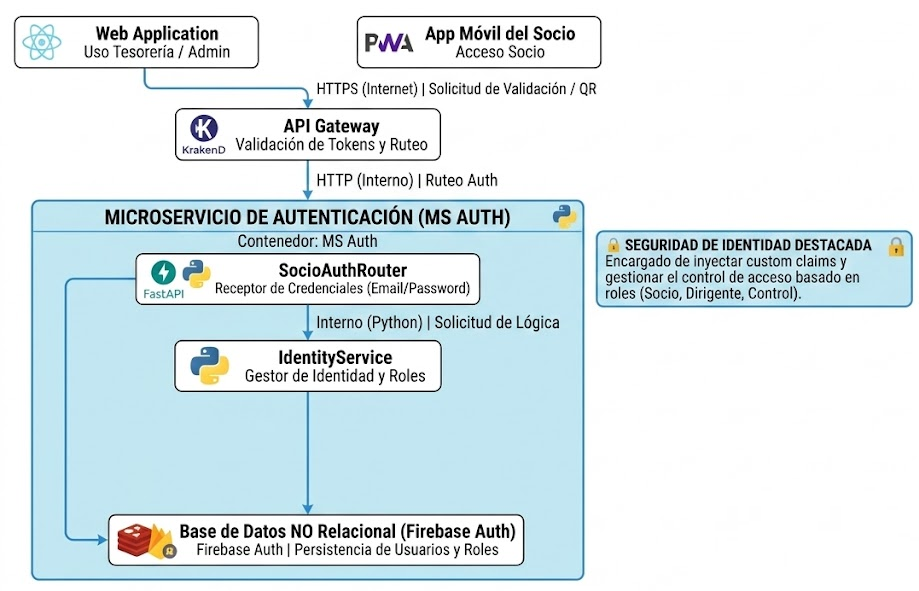
\includegraphics[width=0.95\textwidth]{img/c4_model/C4 Nivel 3-MS Auth.png}
    \caption{Diagrama C4 nivel 3: Componentes (Microservicio de autenticación). Sistema centralizado para el manejo de identidades, validación de credenciales y generación de vales web JSON (Tokens JWT).}
    \label{fig:c4_nivel3_auth}
    
    \vspace{0.2cm} % Espacio vertical de separación entre ambos cuadros

    % Segundo: Componentes (MS Analytics & AI)
    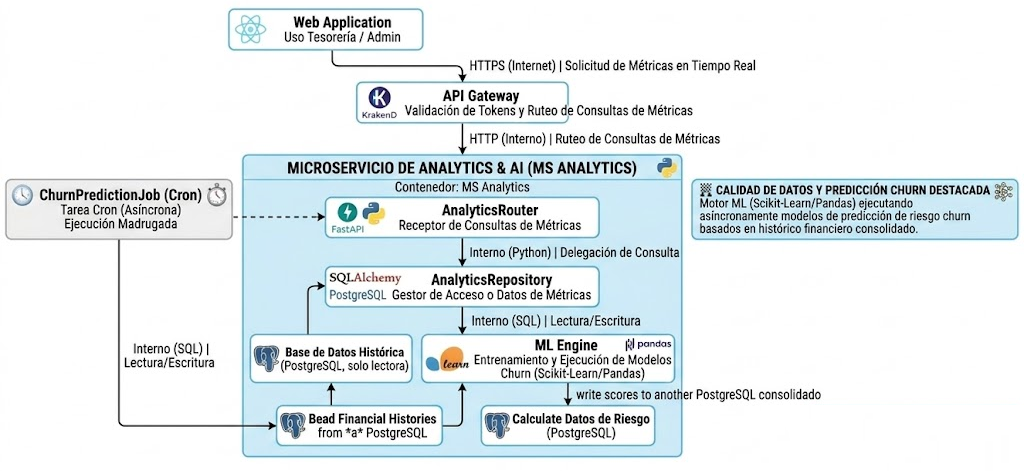
\includegraphics[width=0.95\textwidth]{img/c4_model/C4 Nivel 3-MS Analytics & AI.png}
    \caption{Diagrama C4 nivel 3: Componentes (Microservicio de analítica e inteligencia artificial). Orquestación de tareas asíncronas y motor de \textit{aprendizaje automático (Machine Learning)} para la predicción de riesgo de morosidad.}
    \label{fig:c4_nivel3_analytics}
\end{figure}
